\documentclass[12pt]{article}

\usepackage{graphicx}
\usepackage{paralist}
\usepackage{amsfonts}
\usepackage{amsmath}
\usepackage{hhline}
\usepackage{booktabs}
\usepackage{multirow}
\usepackage{multicol}
\usepackage{url}
\usepackage{hyperref}

\oddsidemargin -10mm
\evensidemargin -10mm
\textwidth 160mm
\textheight 200mm
\renewcommand\baselinestretch{1.0}

\pagestyle {plain}
\pagenumbering{arabic}

\newcounter{stepnum}

%% Comments

\usepackage{color}

\newif\ifcomments\commentstrue

\ifcomments
\newcommand{\authornote}[3]{\textcolor{#1}{[#3 ---#2]}}
\newcommand{\todo}[1]{\textcolor{red}{[TODO: #1]}}
\else
\newcommand{\authornote}[3]{}
\newcommand{\todo}[1]{}
\fi

\newcommand{\wss}[1]{\authornote{blue}{SS}{#1}}

\title{Assignment 4, Specification}
\author{SFWR ENG 2AA4}

\begin {document}

\maketitle
The following Module Interface Specification document provides the modules, types and methods needed to create the game 2048. Once \verb|make main| is typed into the terminal, a grid of 4-by-4 is printed onto the screen, along with instructions to navigate the game. The grid consists of 2 values, each being either a 2 or a 4, with the remaining 14 tiles initialized as 0. The user can use four keys to indicate the direction in which they would like to move; entering i moves the tiles up, entering k moves  the tiles down, entering j moves the tiles left, and entering l moves the tiles right. Once the tiles move at the user’s command, any tile adjacent to another in that direction is combined with that tile if the two tiles are equal in value, and continue shifting in that direction. The game terminates if a tile on the board has the value of 2048, indicating the user has won. The game also terminates if every tile on the board has a value greater than zero, and no two adjacent tiles have the same value. This indicates that the user has lost. In either case, when the game terminates, the board resets to its initial state. This game uses the \verb|Display| module as the View, the \verb|BoardT| module as the Model, the \verb|Controller| as the Controller, and the \verb|Game| module as a way to use \verb|BoardT| based on user input from \verb|Controller|.

\section* {Likely Changes}
\begin{itemize}
  \item The visual representation of the game such as UI layout
  \item The hardware on which the game is run
  \item The constraints on the input parameters
\end{itemize} 

% In applying the specification, there may be cases that involve undefinedness.
% We will interpret undefinedness following~\cite{Farmer2004}:

% If $p: \alpha_1 \times .... \times \alpha_n \rightarrow \mathbb{B}$ and any of
% $a_1, ..., a_n$ is undefined, then $p(a_1, ..., a_n)$ is False.  For instance,
% if $p(x) = 1/x < 1$, then $p(0) = \text{False}$.  In the language of our
% specification, if evaluating an expression generates an exception, then the
% value of the expression is undefined.

% \wss{The parts that you need to fill in are marked by comments, like this one.
%   In several of the modules local functions are specified.  You can use these
%   local functions to complete the missing specifications.}

% \wss{As you edit the tex source, please leave the \texttt{wss} comments in the
%   file.  Put your answer \textbf{after} the comment.  This will make grading
%   easier.}

% \bibliographystyle{plain}
% \bibliography{SmithCollectedRefs}

\newpage

\section* {Display Module}

\subsection*{Module}

Display

\subsection* {Uses}

None

\subsection* {Syntax}

\subsubsection* {Exported Constants}

None

\subsubsection* {Exported Types}

None

\subsubsection* {Exported Access Programs}

\begin{tabular}{| l | l | l | p{5cm} |}
\hline
\textbf{Routine name} & \textbf{In} & \textbf{Out} & \textbf{Exceptions}\\
\hline
print & seq of seq of $\mathbb{N}$ & & \\
\hline
introMessage & & & \\
\hline
intructions & & & \\
\hline
prompt & & & \\
\hline
errorMessage & & & \\
\hline
winMessage & & & \\
\hline
loseMessage & & & \\
\hline
\end{tabular}

\subsection* {Semantics}

\subsubsection* {State Variables}

None

\subsubsection* {State Invariant}

None

\subsubsection* {Assumptions}

None

\subsubsection* {Considerations}

\subsubsection* {Access Routine Semantics}

\noindent print($\mathit{board}$):
\begin{itemize}
\item Print the board in 4 by 4 grid, incrementing rows from left to right and incrementing columns top bottom. Include sufficient space between each value.
\end{itemize} 

\noindent introMessage():
\begin{itemize}
\item Print out the message "Welcome! Can you reach 2048?"
\end{itemize} 

\noindent instructions():
\begin{itemize}
\item Print out the message "Use 'i=up', 'k=down', 'j=left', 'l=right'"
\end{itemize} 

\noindent promtp():
\begin{itemize}
\item Print out the message "Which direction?"
\end{itemize} 

\noindent errorMessage():
\begin{itemize}
\item Print out the message "Sorry! Invalid Input! Please use 'i', 'j', 'k', or 'l'"
\end{itemize} 

\noindent winMessage():
\begin{itemize}
\item Print out the message "Congrats, you won!!"
\end{itemize} 

\noindent loseMessage():
\begin{itemize}
\item Print out the message "Uh oh! Try again!"
\end{itemize} 

\newpage

\section* {BoardT}

\subsection*{Template Module}

BoardT

\subsection* {Uses}

None

\subsection* {Syntax}

\subsubsection* {Exported Constants}

\textit{span}:$\mathbb{N}$

\subsubsection* {Exported Types}

BoardT = ?

\subsubsection* {Exported Access Programs}

\begin{tabular}{| l | l | l | p{5cm} |}
  \hline
  \textbf{Routine name} & \textbf{In} & \textbf{Out} & \textbf{Exceptions}\\
  \hline
  new BoardT & & & \\
  \hline
  getGrid & & seq of seq of $\mathbb{N}$& \\
  \hline
  getScore & & $\mathbb{N}$ & \\
  \hline
  newGrid & & & \\
  \hline
  newNumber & & & \\
  \hline
  wonGame & & $\mathbb{B}$ & \\
  \hline
  lostGame & & $\mathbb{B}$ & \\
  \hline
  up & & & \\
  \hline
  down & & & \\
  \hline
  left & & & \\
  \hline
  right & & & \\
  \hline 
  move & String & & \\
  \hline
  add & String & & \\
  \hline  
\end{tabular}

\subsection* {Semantics}

\subsubsection* {State Variables}

$\mathit{score}$: $\mathbb{N}$\\
$\mathit{grid}$: seq of seq of $\mathbb{N}$

\subsubsection* {State Invariant}

None

\subsubsection* {Assumptions}

There is access to a function random that returns number between 0 and 1 

\subsubsection* {Access Routine Semantics}

\noindent new BoardT():
\begin{itemize}
\item transition: $grid, score = \langle i : \mathbb{N} | i \in [0..span-1]: \langle j  : \mathbb{N} | j \in [0..span-1]: 0 \rangle\rangle$, 0,
\item output: $out := self$ 
\item exception: none
\end{itemize}

\noindent getGrid():
\begin{itemize}
\item output: $out := grid$
\item exception: none
\end{itemize}

\noindent getScore():
\begin{itemize}
\item output: $out := score$
\item exception: none
\end{itemize}

\noindent newGrid( ):
\begin{itemize}
\item \mbox{newNumber()}
\item \mbox{newNumber()}
\end{itemize}

\noindent newNumber():
\begin{itemize}
\item transition: \newline
      initialize boolean empty = true \newline
      while empty = true: \newline
      $~~$ initialize integer i = random number  between 0 and 1 multiplied by 4 \newline
      $~~$ initialize integer j = random number  between 0 and 1 multiplied by 4 \newline
      $~~$ initialize double k = random number between 0 and 1 \newline
      $~~$ if grid cell of row i and column j has value of 0: \newline
      $~~$$~~$ if k is less than 0.1: \newline
      $~~$$~~$$~~$ grid cell of row i and column j = 4 \newline
      $~~$$~~$$~~$ empty = false \newline
      $~~$$~~$ else: \newline 
      $~~$$~~$$~~$ grid cell of row i and column j = 2 \newline
      $~~$$~~$$~~$ empty = false; \newline
\end{itemize}

\noindent wonGame():
\begin{itemize}
\item $output: \langle i : \mathbb{N} | i \in [0..span-1]: \langle j  : \mathbb{N} | j \in [0..span-1]| grid[i][j] = 2048 \Rightarrow True| True \Rightarrow False\rangle\rangle$,
\end{itemize}

\noindent lostGame():
\begin{itemize}
\item transition:\newline
      for i in grid length:\newline
      $~~$ for j in grid length:\newline
      $~~$$~~$ if cell at row i column j has a value of 0:\newline
      $~~$$~~$$~~$ return false\newline
      $~~$$~~$ if the cell above cell at row i column j has the same value:\newline
      $~~$$~~$$~~$ return false\newline
      $~~$$~~$ if the cell below cell at row i column j has the same value:\newline
      $~~$$~~$$~~$ return flase\newline
      $~~$$~~$ if the cell to the left of cell at row i column j has the same value:\newline
      $~~$$~~$$~~$ return false\newline
      $~~$$~~$ ig the cell to the right of cell at row i column j has the same value:\newline
      $~~$$~~$$~~$ return false\newline
      return true;\newline
\end{itemize}

\noindent up():
\begin{itemize}
\item \mbox{move("i")}
\item \mbox{add("i")}
\item \mbox{move("i")}
\end{itemize}

\noindent down():
\begin{itemize}
\item \mbox{move("k")}
\item \mbox{add("k")}
\item \mbox{move("k")}
\end{itemize}

\noindent left():
\begin{itemize}
\item \mbox{move("j")}
\item \mbox{add("j")}
\item \mbox{move("j")}
\end{itemize}

\noindent right():
\begin{itemize}
\item \mbox{move("l")}
\item \mbox{add("l")}
\item \mbox{move("l")}
\end{itemize}

\noindent move(direction):
\begin{itemize}
\item Move each cell up if direction is equal to "i", down if direction is equal to "k", left if direction is equal to "j", or right if direction is equal to "l". it iterates through the cells of the grid by incrementing the row and column values. Rightmost cells cannot move right, the leftmost cells cannot move left, the topmost cells cannot move up and the bottommost cells cannot move down. Cells move over only if the adjacent cell in that direction is equal to 0, to avoid overwriting previously existing values. Each time the cell moves over, its previous position is overwritten to become zero. Each cell must be moved as far is it can be moved in the specified direction.
\end{itemize}

\noindent add(direction):
\begin{itemize}
\item If the specified direction is "i", iterate through each cell, starting from the second row and the first column, and compare it to the cell above. If their values are equal, overwrite the value of the cell above  to be the sum of their values. Add to the score the sum of the values. Overwrite the current cell to become zero. \newline
If the specified direction is "k", begin at the third row and first column, and iterate through the cells, decrementing the row and incrementing the column. Compare each cell to the one below it; if their values are equal, overwrite the value of the cell below to be the sum of their values. Add to the score the sum of the values. Overwrite the value of the current cell to become 0. \newline
If the specified direction is "j", iterate through each cell, starting from the first row and the second column. Increment the row and column each time. Compare the value of each cell to the left adjacent column.   If their values are equal, overwrite the value of the left cell to be the sum of their values. Add to the score the sum of the values. overwrite the current cell's value to be 0. \newline
If the specified direction is "l" begin at the first row and third column and iterate through each cells, incrementing the row and decrementing the column. Compare the current cell's value to the value of the right adjacent cell's value; if they are equal, overwrite the right adjacent value to become the sum of both values. Add to the score the sum. Overwrite the current cell's value to be 0. 
\end{itemize}

\newpage

\section* {Controller Module}

\subsection*{Module}

Controller

\subsection* {Uses}

Game \newline
Display

\subsection* {Syntax}

\subsubsection* {Exported Constants}

None

\subsubsection* {Exported Types}

None

\subsubsection* {Exported Access Programs}

\begin{tabular}{| l | l | l | p{5cm} |}
\hline
\textbf{Routine name} & \textbf{In} & \textbf{Out} & \textbf{Exceptions}\\
\hline
getUserInput & & & \\
\hline
runGame & & & \\
\hline
\end{tabular}

\subsection* {Semantics}

\subsubsection* {Environment Variables}

\textit{input}:Scanner

\subsubsection* {State Variables}

None

\subsubsection* {State Invariant}

None

\subsubsection* {Assumptions}

None

\subsubsection* {Access Routine Semantics}

\noindent getUserInput():
\begin{itemize}
\item transition: \newline
      \mbox{prompt()} \newline
      initialize Scanner input = \mbox{new Scanner} \newline
      initialize string direction = next line input \newline
      if direction $\neq$ "i" and $\neq$ "k" and $\neq$ "j" and $\neq$ "l": \newline
      $~~$ \mbox{errorMessage()}\newline
      else \newline
      $~~$ \mbox{whereToGo(direction)} \newline
\end{itemize} 

\noindent runGame():
\begin{itemize}
\item transition: \newline
      \mbox{introMessage()} \newline
      Print a new line \newline
      \mbox{instructions()}; \newline
      \mbox{resetGame()}; \newline
      while true: \newline
      $~~$ print the game board \newline
      $~~$ \mbox{getUserInput} \newline
\end{itemize} 

\newpage

\section* {Game Module}

\subsection*{Module Module}

Game

\subsection* {Uses}

Controller \newline
BoardT \newline
Display
\subsection* {Syntax}

\subsubsection* {Exported Constants}

None

\subsubsection* {Exported Types}


\subsubsection* {Exported Access Programs}

\begin{tabular}{| l | l | l | p{5cm} |}
\hline
\textbf{Routine name} & \textbf{In} & \textbf{Out} & \textbf{Exceptions}\\
\hline
getBoard & & BoardT & \\
same & seq of seq of $\mathbb{N}$ & seq of seq of $\mathbb{N}$ & \\
\hline
whereToGo & String & & ~\\
\hline
resetGame & & & ~\\
\hline
checkGameStatus & & & \\
\hline
\end{tabular}

\subsection* {Semantics}

\subsubsection* {State Variables}

$\mathit{b}: \text{BoardT}$\\

\subsubsection* {State Invariant}

None

\subsubsection* {Assumptions}

\verb|resetGame()| is called before any other Access Routine in the module

\subsubsection* {Access Routine Semantics}

\noindent getBoard():
\begin{itemize}
\item output: $out := b$ 
\item exception: none
\end{itemize}

\noindent same($grid$):
\begin{itemize}
\item output: $out := \langle i : \mathbb{N} | i \in [0..grid-1]: \langle j  : \mathbb{N} | j \in [0..grid-1]: grid[i][j] \rangle\rangle$
\item exception: none
\end{itemize}

\noindent whereToGo($direction$):
\begin{itemize}
\item transition \newline
      initialize double array b = \mbox{same(\textit{b})} \newline
      if direction = "i": \newline
      $~~$\textit{b}.\mbox{up()} \newline
      else if direction = "k": \newline
      $~~$  \textit{b}.\mbox{down()} \newline
      else if direction = "j": \newline
      $~~$ \textit{b}.\mbox{left()} \newline
      else if direction = "l": \newline
      $~~$ \textit{b}.\mbox{right()} \newline
      initialize double array a = \mbox{same(\textit{b})} \newline
      if a $\neq$ b: \newline
      $~~$  \textit{b}.\mbox{newNumber()} \newline
      \mbox{checkGameStatus} \newline
\item exception: none
\end{itemize}

\noindent resetGame():
\begin{itemize}
\item transition: $b := new \mbox{BoardT}$
\item \textit{b}.\mbox{newGrid()}
\end{itemize}

\noindent checkGameStatus():
\begin{itemize}
\item transition: \newline
      if \textit{b}.\mbox{wonGame()}: \newline
      $~~$ \mbox{winMessage()} \newline
      $~~$ \mbox{resetGame()} \newline
      else if \textit{b}.\mbox{lostGame()} \newline
      $~~$ \mbox{loseMessage()} \newline
      $~~$ \mbox{resetGame()} \newline
\end{itemize}
\newpage

\section* {Critique}
$~~$$~~$$~~$$~~$The implementation of my design ensures minimality within each module, in that no two methods accomplish the same computation and outputs. This adds to the quality of essentiality, as every method created within the design is used and necessary for the performance of the game. This was not the case during the entirety of the design process. I had initially created a method \verb|full()| which served to check if every value on the grid was greater than 0. This used a nested for loop to iterate through the rows and columns and a counter, which was incremented for every value in the grid that was greater than 0. If the counter by the end was equal to 16 by the end of the iteration, the method would return a boolean value ‘true’, or else it would return ‘false’. Soon into creating the \verb|lostGame()| method, however, I realized I could accomplish the same computation in one simple step, and so the \verb|full()| method omitted from the \verb|BoardT| module. In doing so, BoardT has a great quality of minimality and essentiality, by reducing time complexity and an entire method that was not actually necessary. \newline
\newline
$~~$$~~$$~~$$~~$The MIS for each module is general in that it specifies only what needs to be outputted, but is open ended for the developer to decide how they would wish to implement the methods. For a few methods, however, there is no way to make the specification general; the \verb|up()|, \verb|down()|, \verb|left()|, and \verb|right()| methods call on other methods and thus cannot be implemented in more ways than one. \newline
\newline
$~~$$~~$$~~$$~~$The design is consistent in naming conventions, in that each method with more than one word is named using Camel Case, while one word methods are lowercase. The parameters used for methods are all name consistently; every parameter of type \verb|int[][]| is given the variable name \verb|board|, which is synonymous to \verb|grid| but is used to avoid confusion. Every parameter of type \verb|String| is given the variable name \verb|direction| to make the code easily to follow along with. Iteration through the cells of the grid use the same variables, where \verb|int i| and \verb|int j| represent the row and column of the grid, respectively. The design was created to make errors legible to the user in the form of a displayed message, as opposed to raising an error. If the user input is not equal ‘i’, ‘k’, ‘j’ or ‘l’, the system displays a message informing them that their input is invalid, and that they should use the appropriate keys to navigate the game. By not raising an error for every invalid key pressed, the game does not halt, which allows the user to continue playing and avoids having to restart every time. \newline
\newline
$~~$$~~$$~~$$~~$The design additionally has high cohesion, in that the properties of each module as closely related. They work an accomplish specific things, however in order to run the game, including the controller, the model of the board, and the display of the board and prompt, each module works together. In terms of information hiding, methods used by other modules were made public. The instances of the \verb|BoardT| created were made private to avoid user manipulation. This allows whatever happens with the model of the board based on user input to happen behind the scenes. 


\section* {Question 1}

\begin{center}
  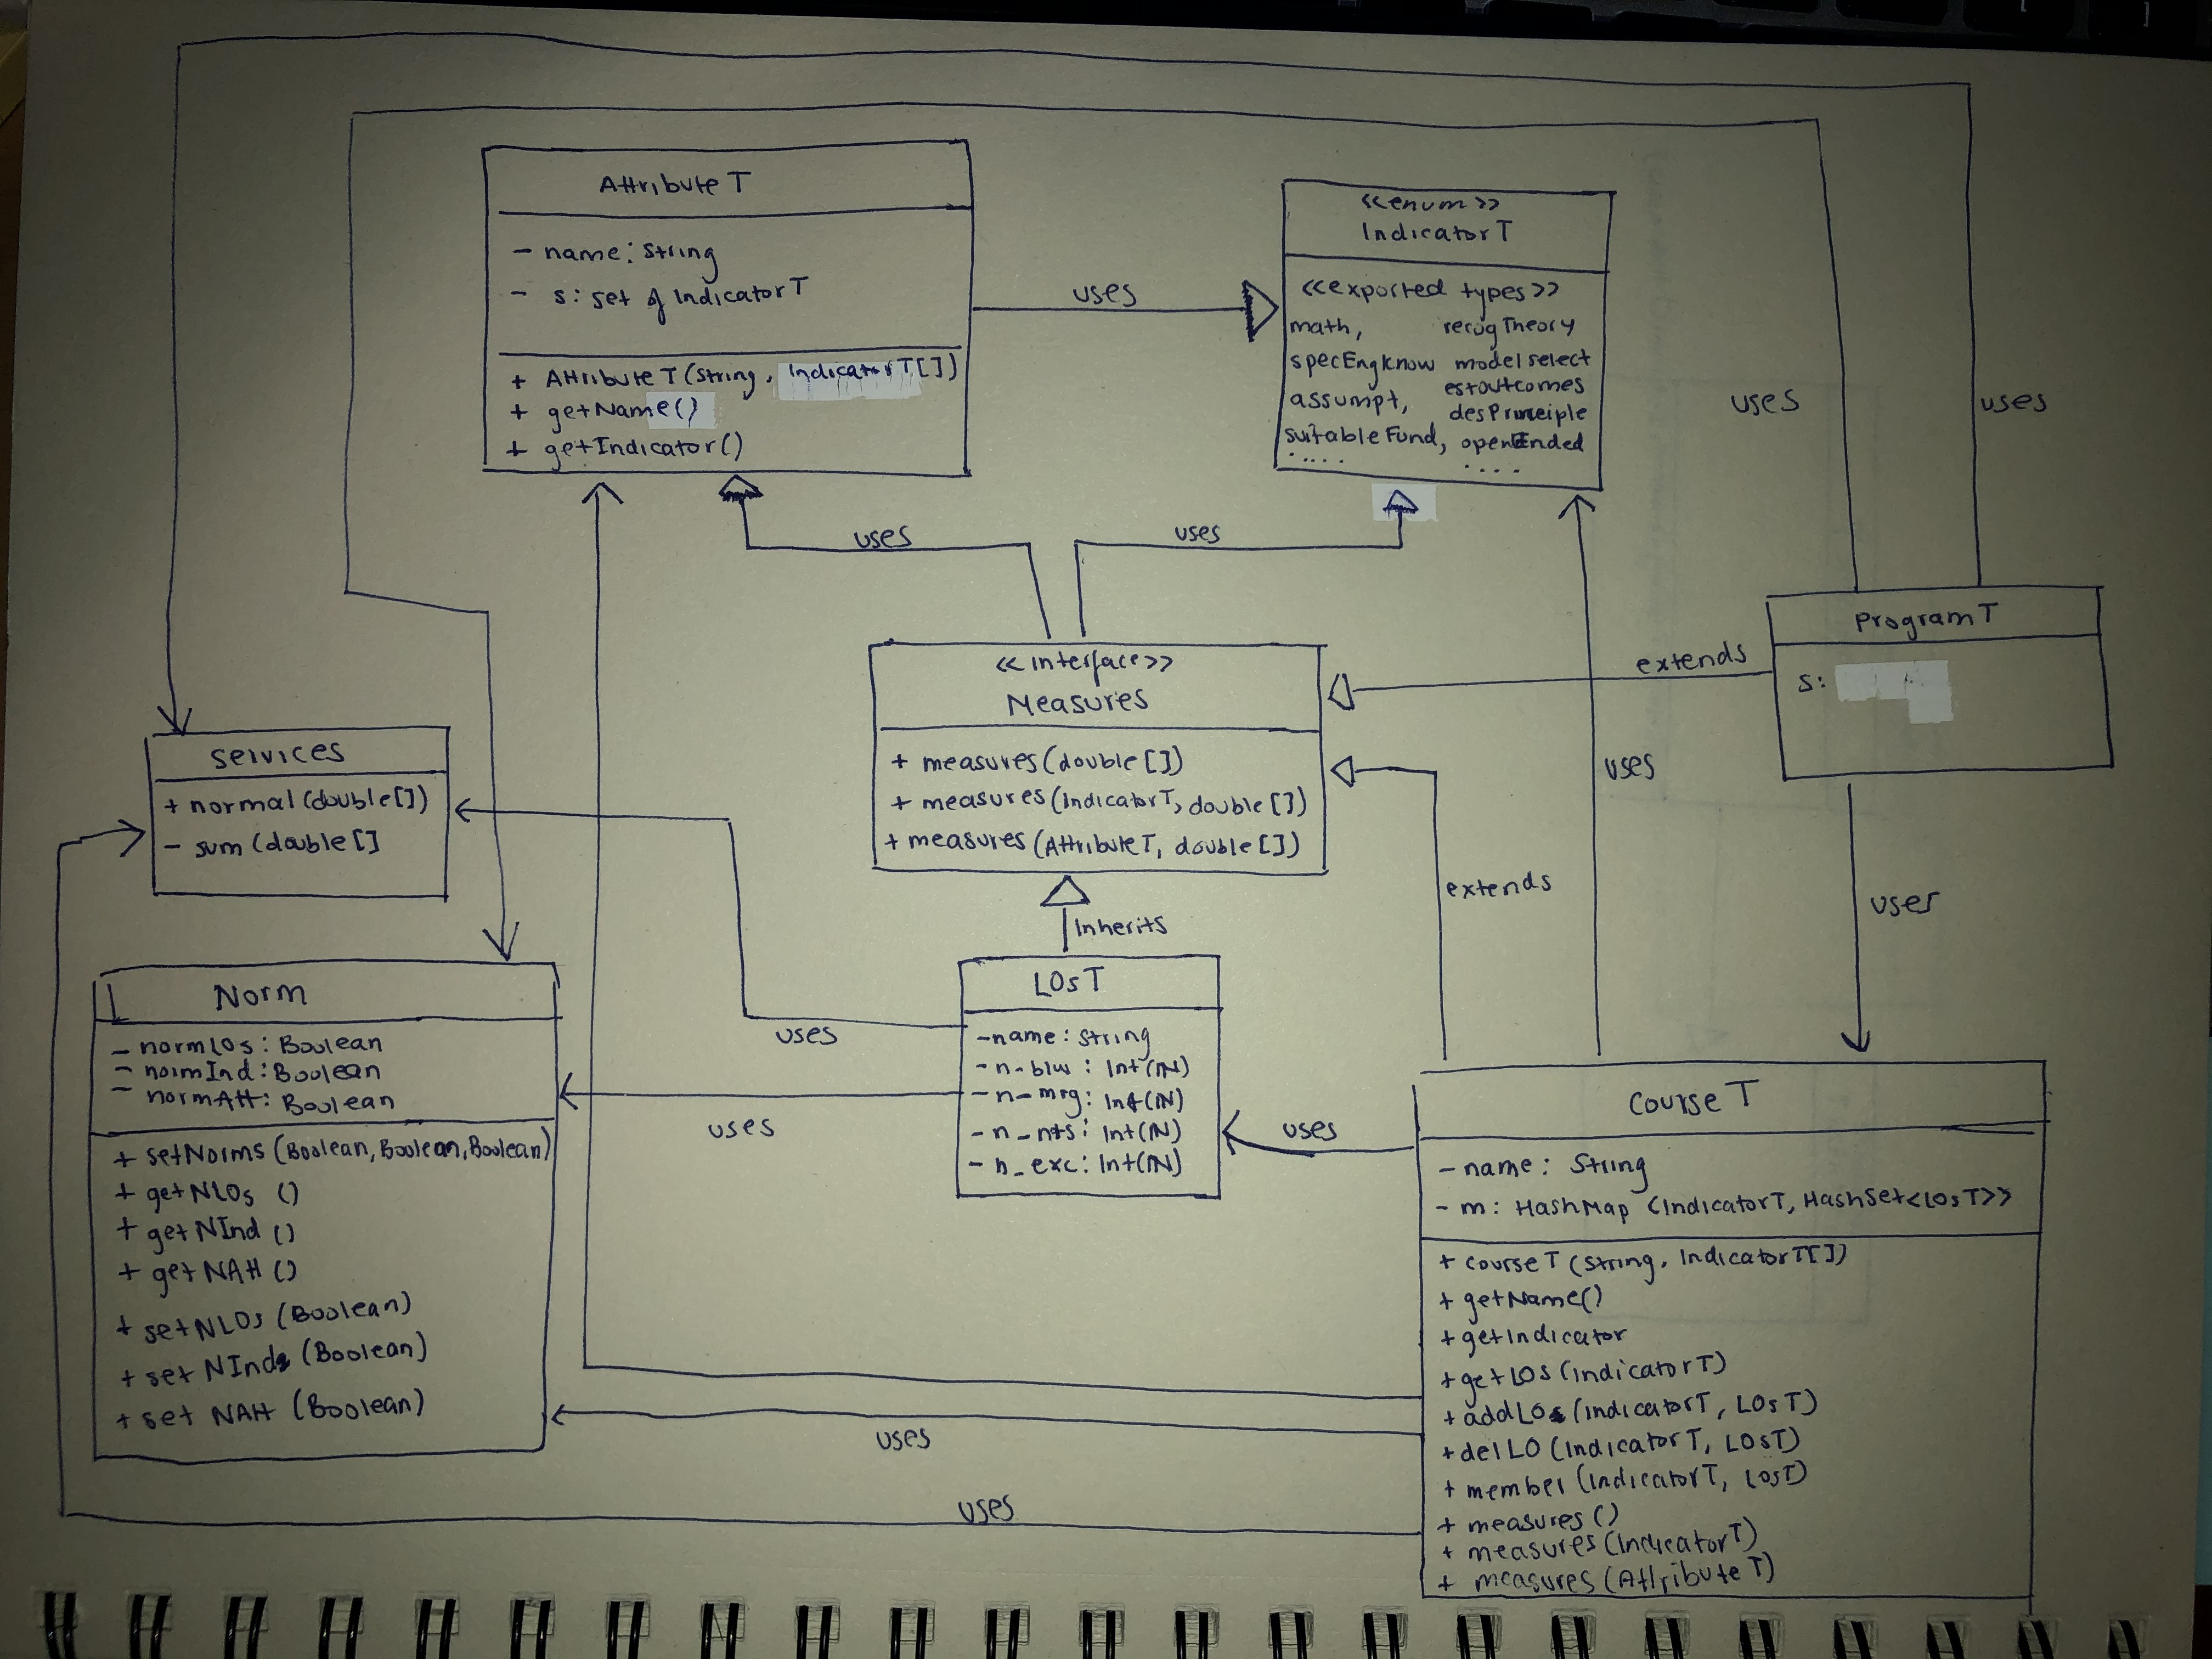
\includegraphics[width=0.8\textwidth]{UML.jpg}
\end{center}

\section* {Question 2}

\begin{center}
  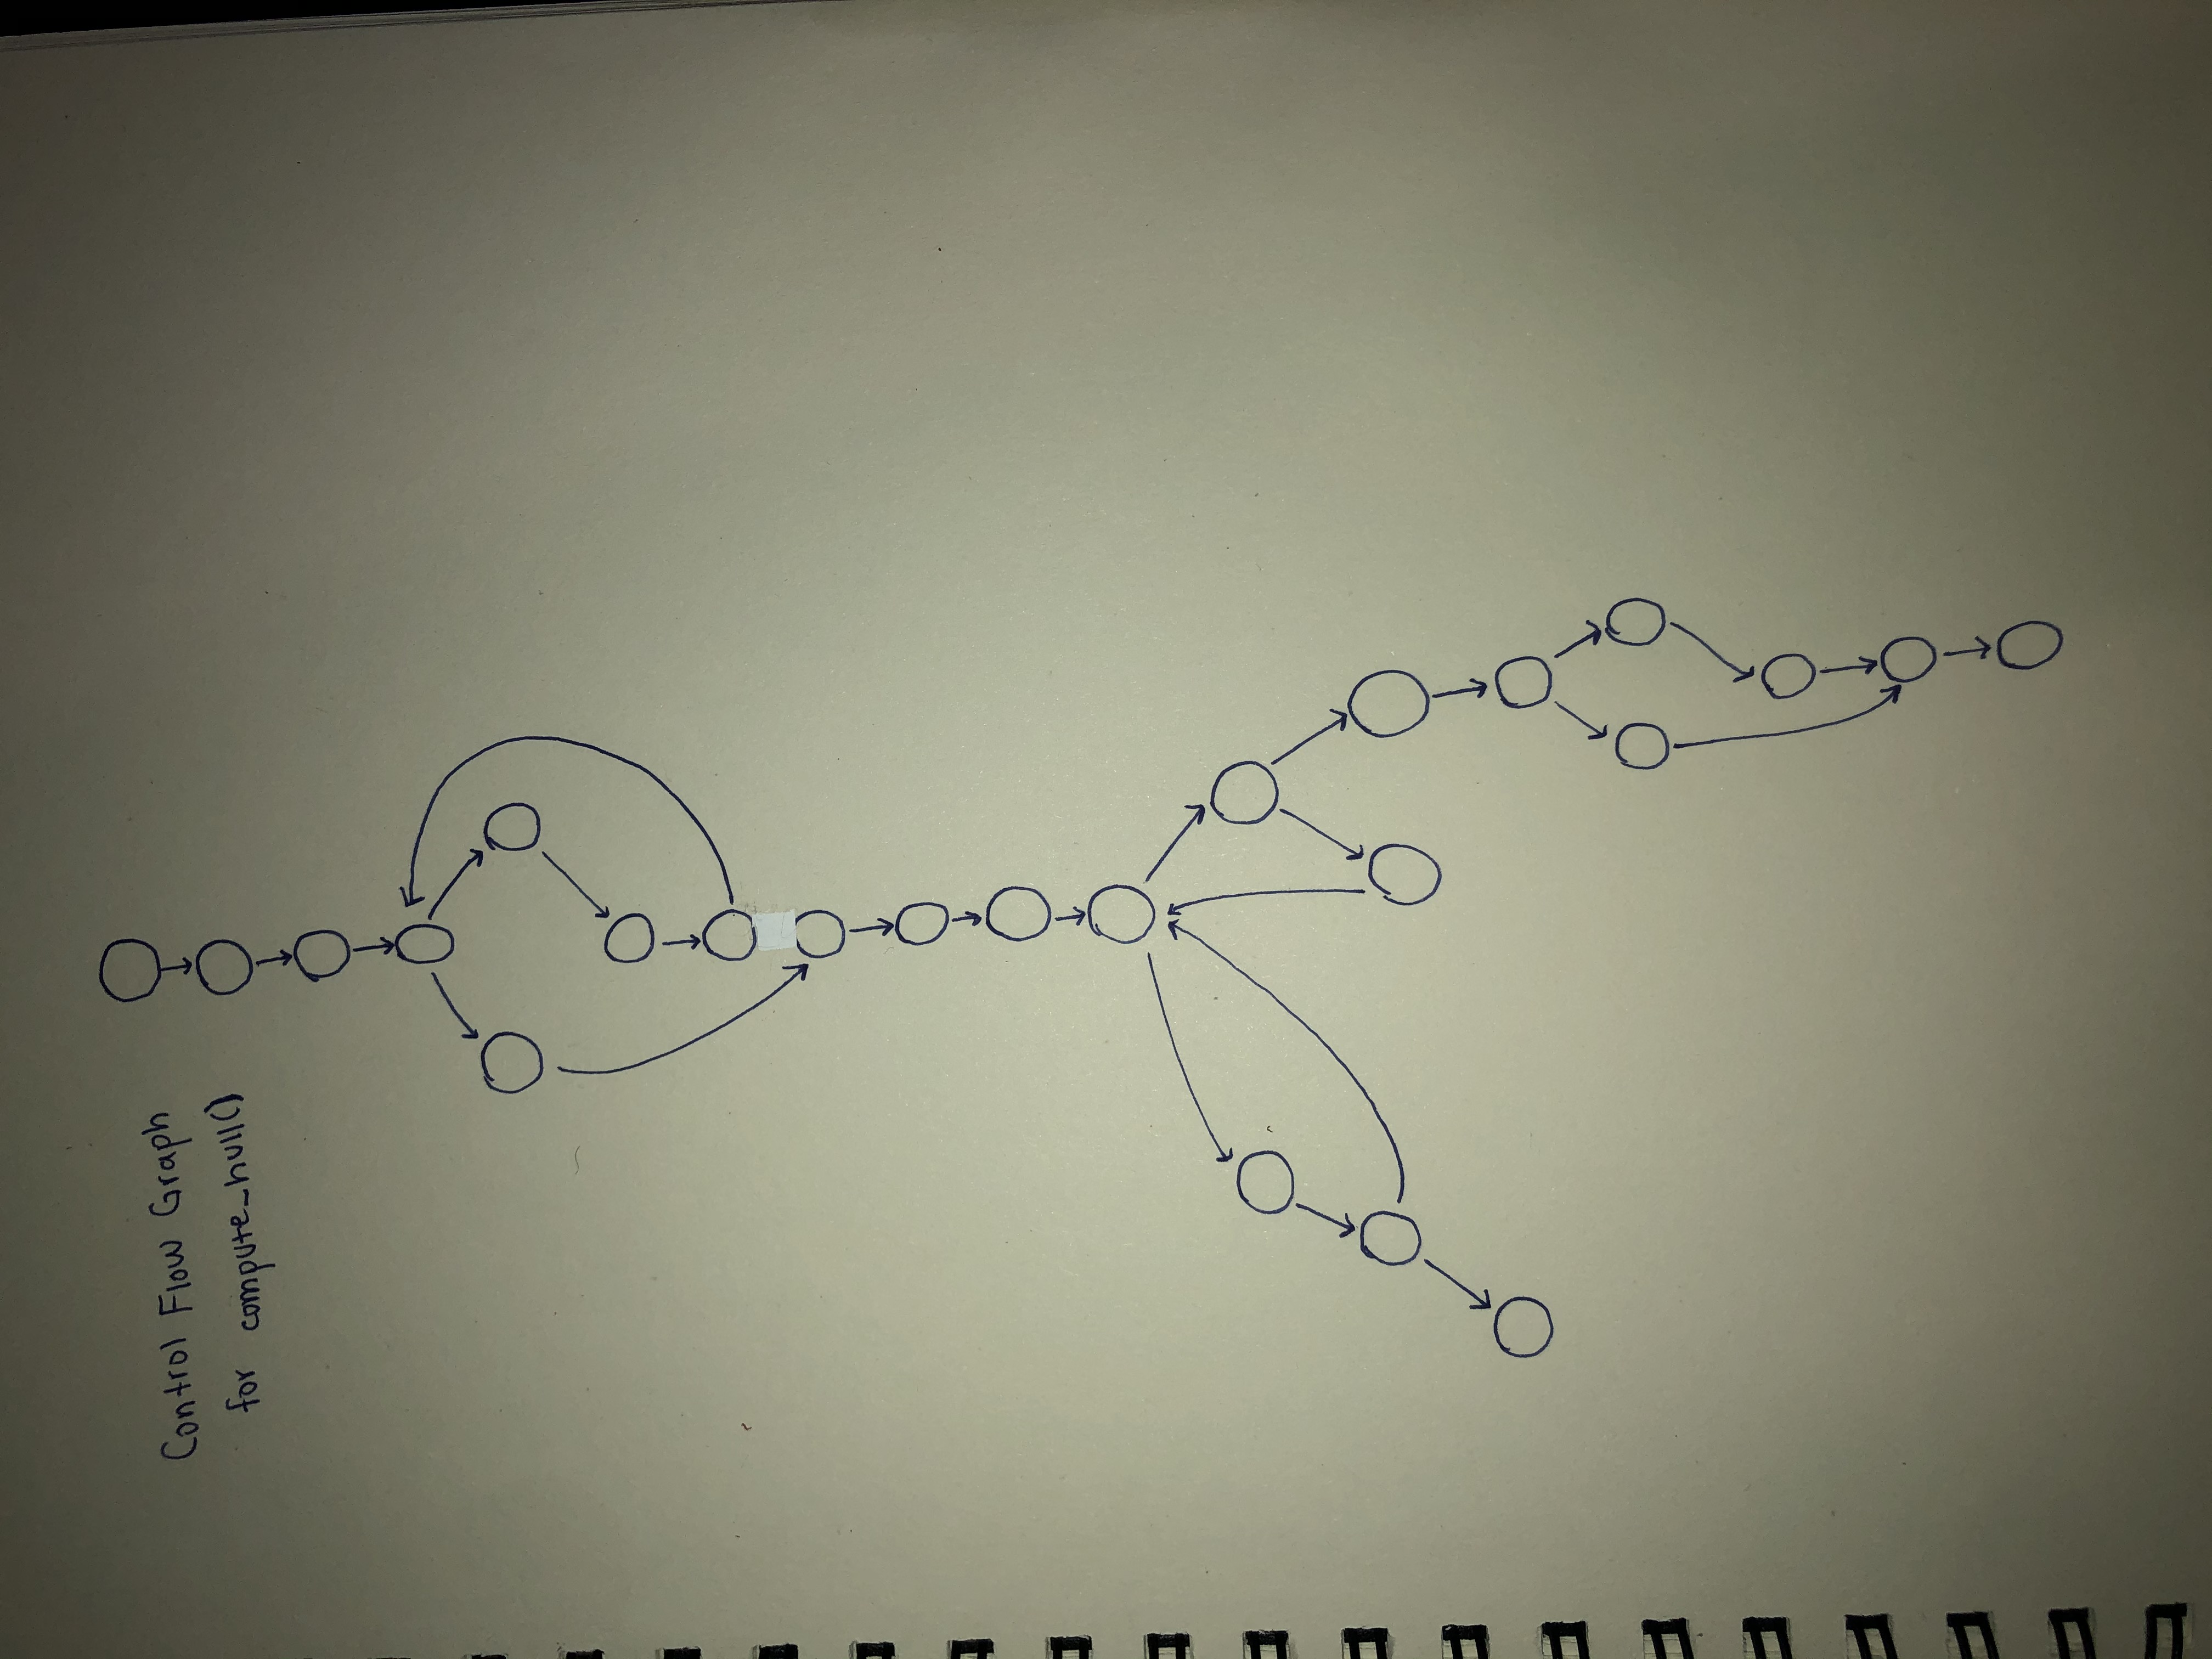
\includegraphics[width=0.8\textwidth, angle = 270]{CFG.jpg}
\end{center}

\end {document}
